\section{R-emo}
  \subsection{Metodología de Desarrollo}
      \begin{frame}\frametitle{\textbf{Metodología de Desarrollo}}
          \begin{center}
            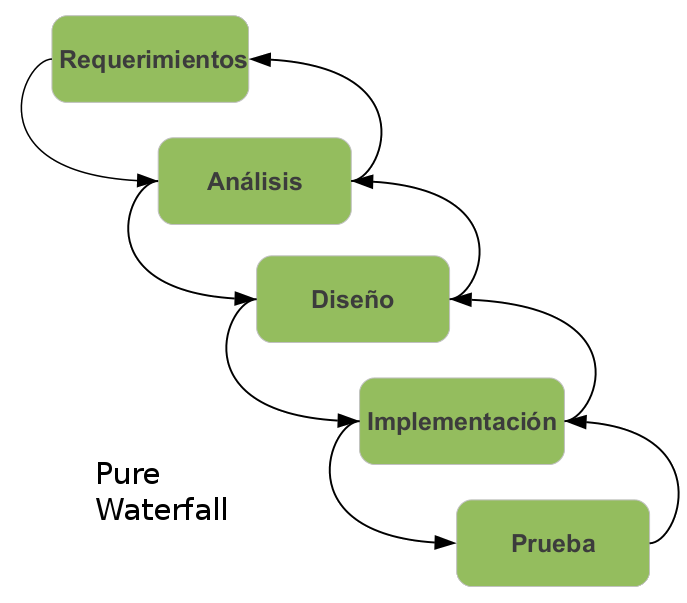
\includegraphics[scale=.4]{images/cascadaPuro.png}
          \end{center}
      \end{frame}  
      
      \begin{frame}\frametitle{\textbf{Consideraciones sobre la Metodología}}
          \begin{center}  
            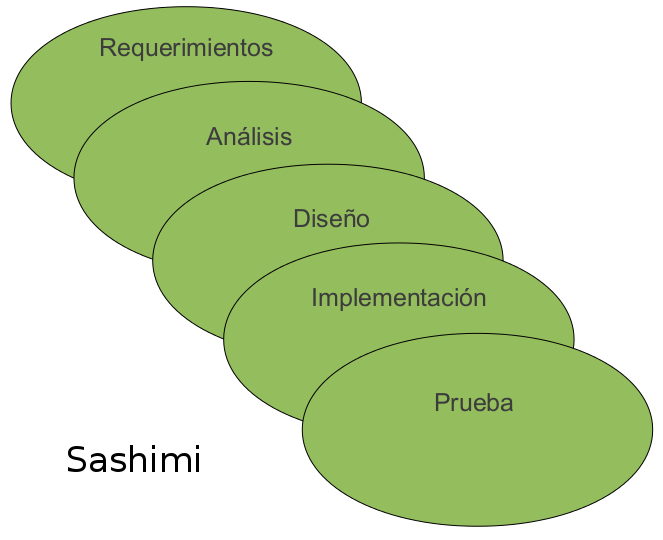
\includegraphics[scale=.42]{images/sashimi2.png}
          \end{center}
      \end{frame}  

      \begin{frame}\frametitle{\textbf{Consideraciones sobre la Metodología (cont.)}}        
          \begin{center}
            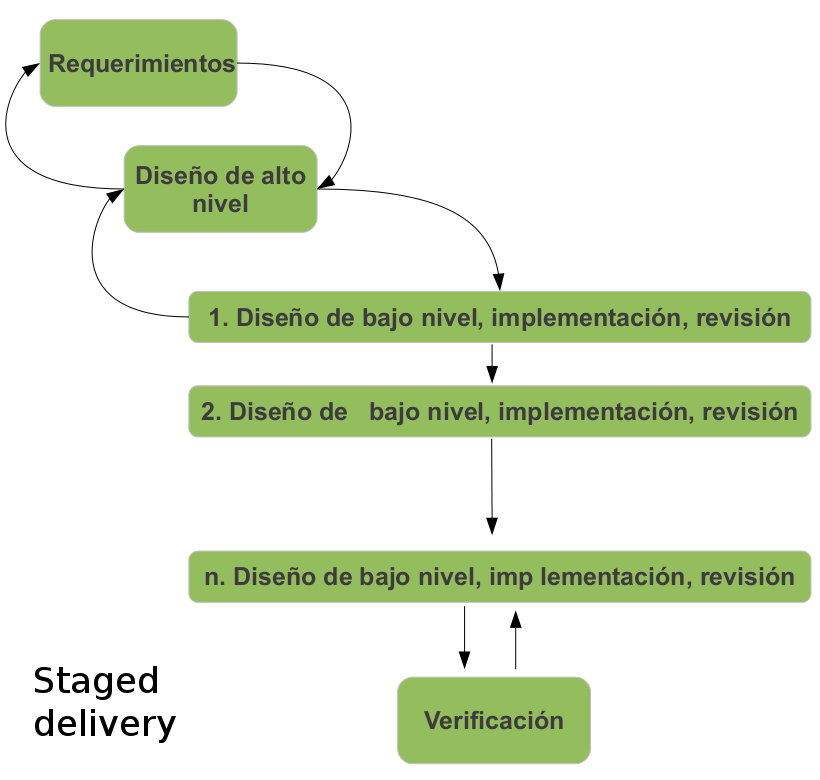
\includegraphics[scale=.35]{images/stagedDelivery2.png}
          \end{center}        
      \end{frame}  

  \subsection{Elicitación y Análisis}
      \begin{frame}\frametitle{\textbf{Especificación}}
        \hspace*{-1cm} 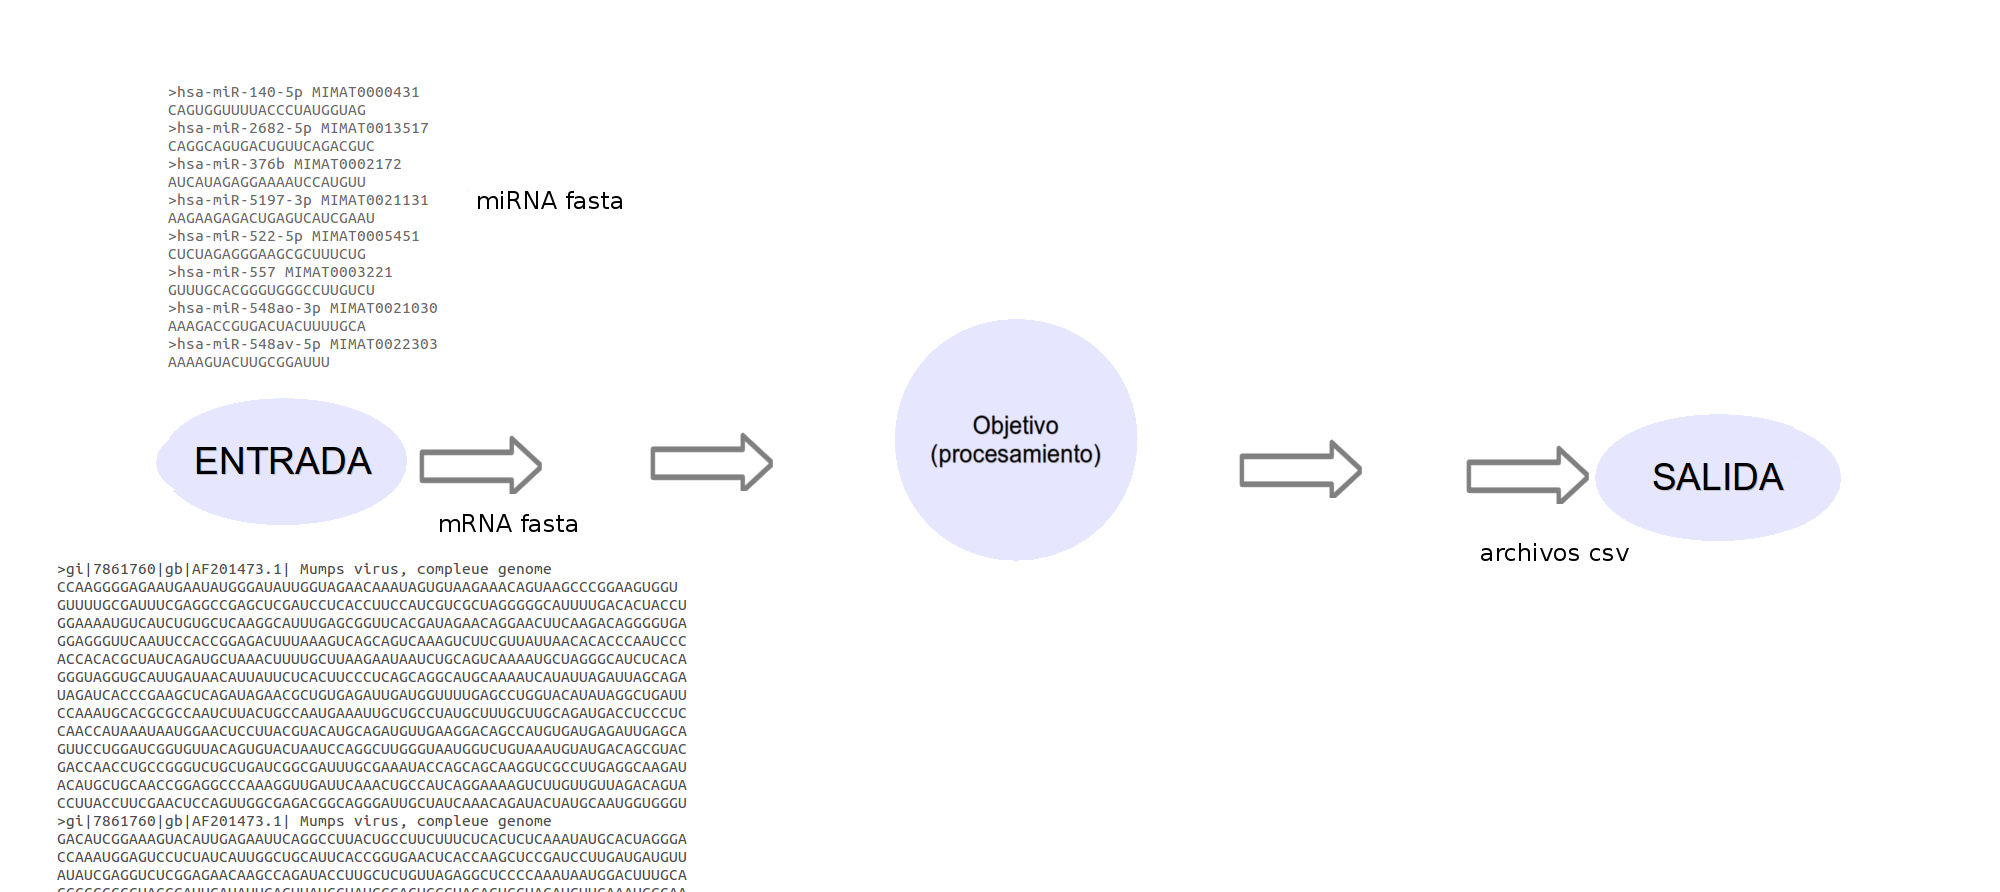
\includegraphics[scale=.19]{images/especificacion1.png}
      \end{frame}  

      \begin{frame}\frametitle{\textbf{Especificación (cont.)}}
        \hspace*{-.9cm}  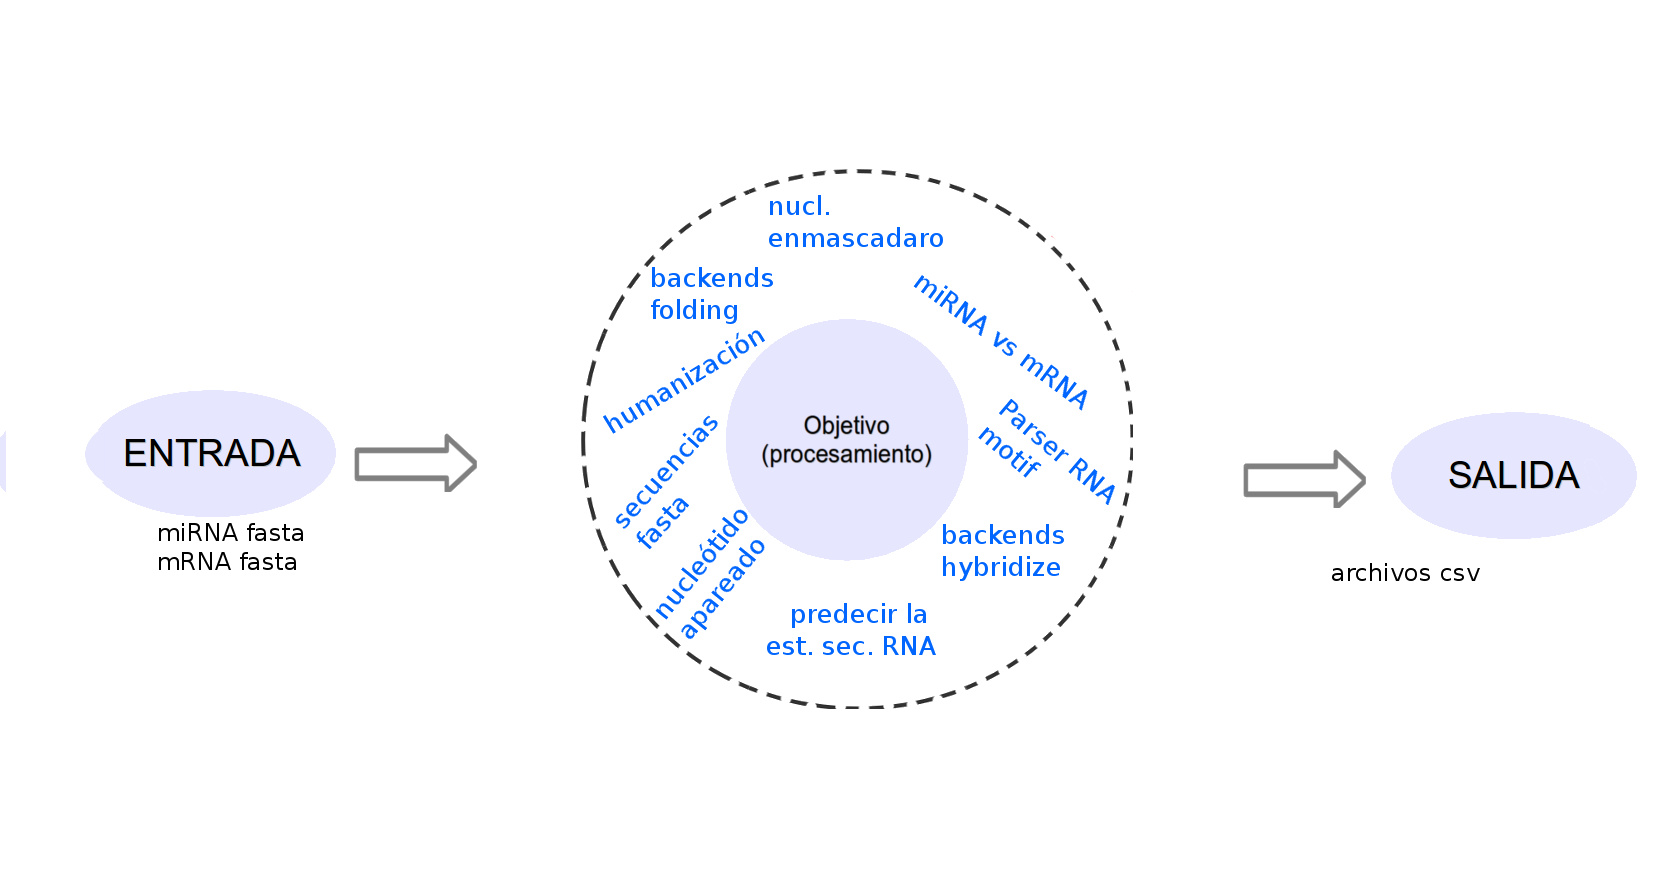
\includegraphics[scale=.2]{images/especificacion2.png}
      \end{frame}  

      \begin{frame}\frametitle{\textbf{Especificación (cont.)}}
        \hspace*{-.5cm} 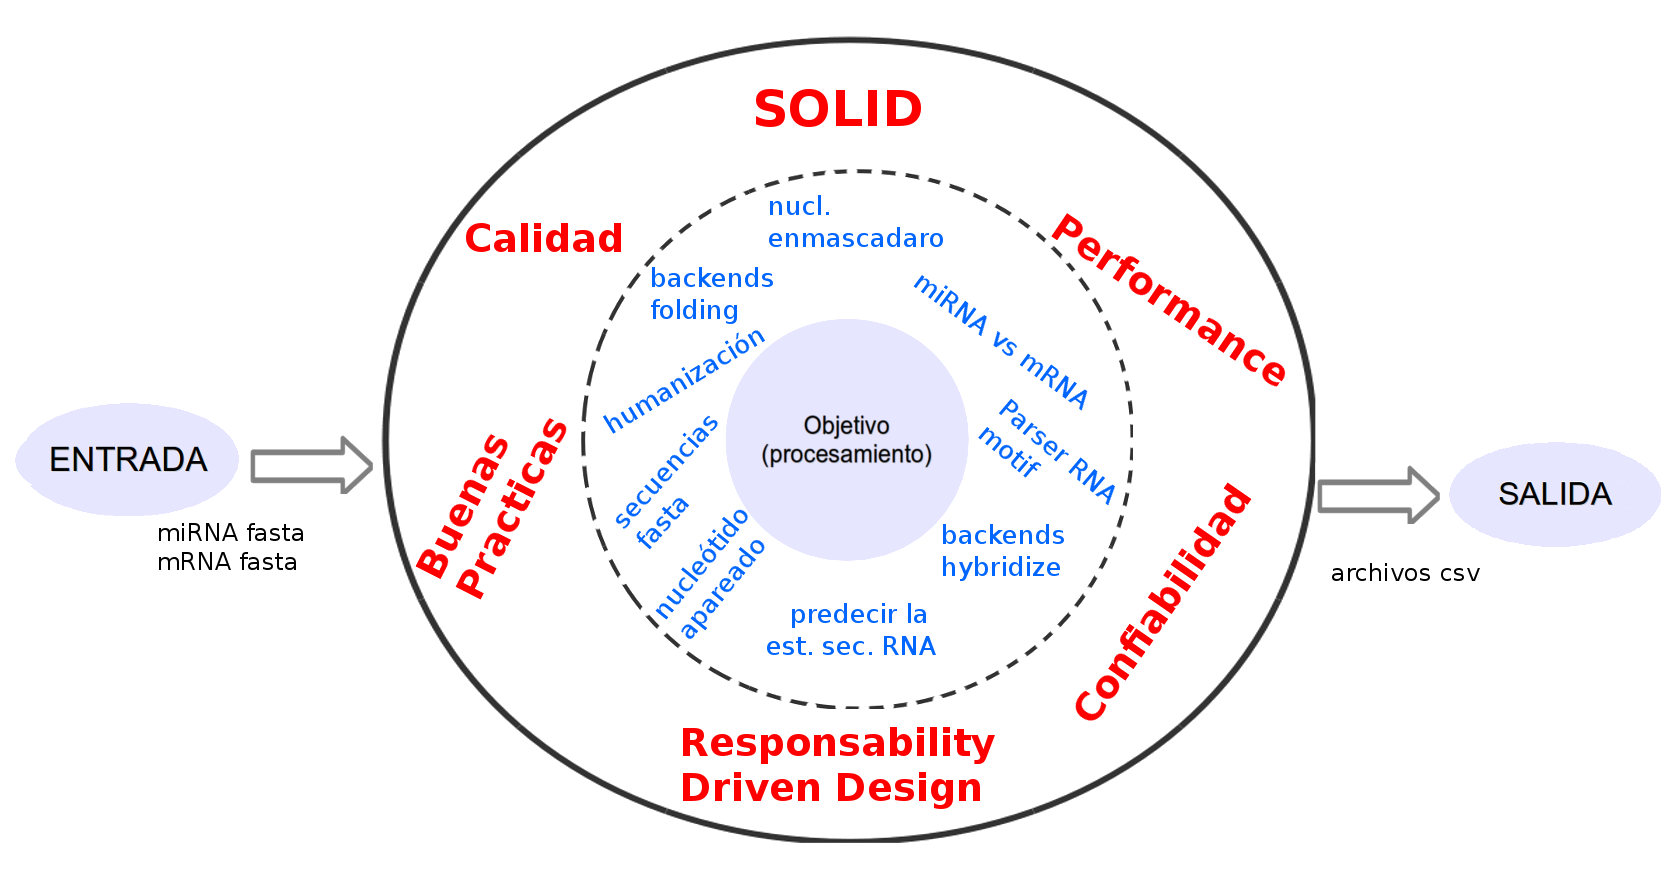
\includegraphics[scale=.2]{images/especificacion3.png}
      \end{frame}  

      \begin{frame}\frametitle{\textbf{Creación de librerías}}
        \begin{block}{Surgen:}
          \begin{itemize}
            \item \textbf{fideo   :} Folding Interface Dynamic Exchange Operations
                \vskip .05cm
                \hspace*{2.9cm}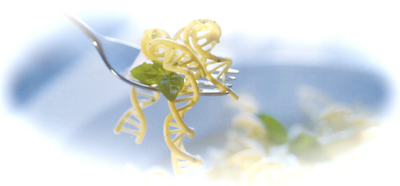
\includegraphics[scale=.2]{images/fideo.png}
            \item \textbf{acuoso  :} Abstract Codon Usage Optimization Software for Organisms
                \vskip .05cm
                \hspace*{3.5cm}
\includegraphics[scale=.3]{images/acuoso.png}
            \item \textbf{etilico :} External Tools Invocation LIbrary and COmponent
                \vskip .05cm
                \hspace*{2.25cm}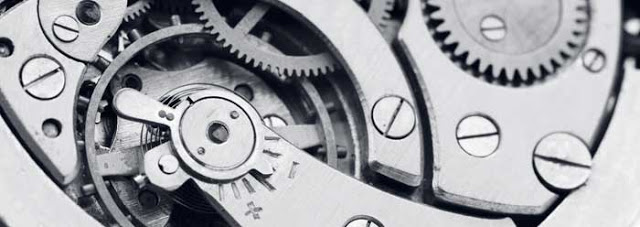
\includegraphics[scale=.19]{images/etilico.jpg}
          \end{itemize}  
        \end{block}  
      \end{frame}  

  \subsection{Diseño}
      \begin{frame}\frametitle{\textbf{Principios de Diseño}}
          \begin{block}{Resposability-Driven Design}
              \begin{minipage}{2cm \textwidth}
                  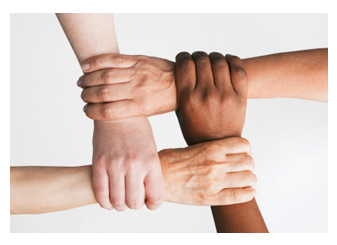
\includegraphics[scale=.2]{images/manos.jpg}
              \end{minipage}
              \begin{minipage}{8cm}
                  \begin{itemize}
                    \item Que responsabilidades debe cubrir el sistema.
                    \item Cuales serán los objetos responsables de llevarlas a cabo.                    
                  \end{itemize}                  
              \end{minipage}           
          \end{block}  

      \begin{block}{SOLID}
      \begin{minipage}{7cm \textwidth}
          \begin{itemize}
            \item   \textbf{S}ingle Responsibility Principle (SRP)
            \item   \textbf{O}pen-Closed Principle (OCP)
            \item   \textbf{L}iskov Substitution Principle (LSP)
            \item   \textbf{I}nterface Segregation Principle (ISP)
            \item   \textbf{D}ependency Inversion Principle (DIP)          
          \end{itemize}            
    \end{minipage}
    \begin{minipage}{3cm}
      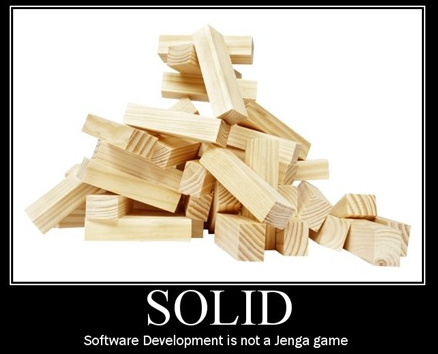
\includegraphics[scale=.3]{images/solid.png}
    \end{minipage}     
    \end{block}         
      \end{frame}  

      \begin{frame}\frametitle{\textbf{Arquitectura}}
        \begin{center}
          %A un alto nivel de componentes
          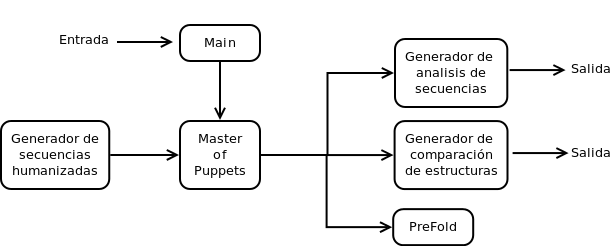
\includegraphics[scale=.4]{images/componenteRemo.png}
        \end{center}
      \end{frame}  

      \begin{frame}\frametitle{\textbf{Arquitectura (refinando)}}
        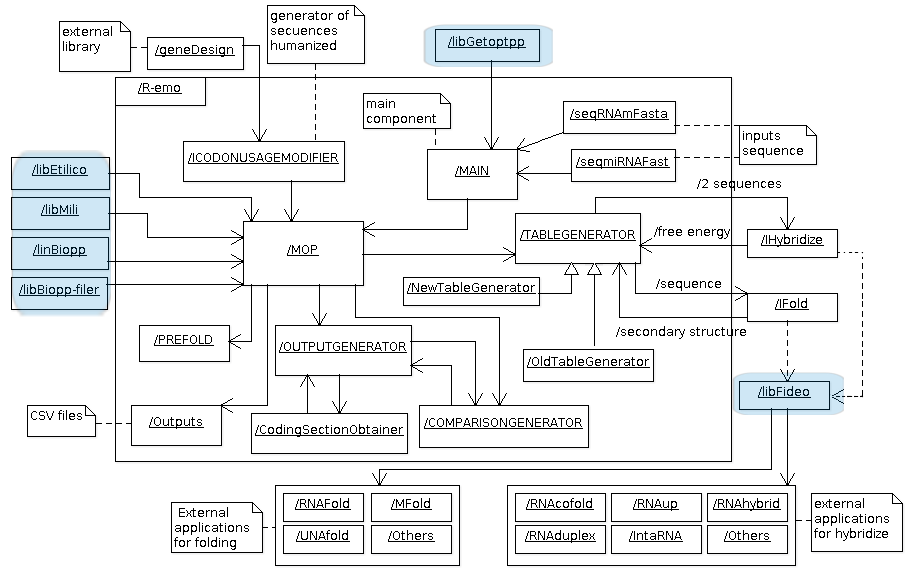
\includegraphics[scale=.35]{images/arquitectura.png}
      \end{frame}  

      \begin{frame}\frametitle{\textbf{Diagrama de Clases}}
        \begin{center}
          
\includegraphics[scale=.25]{images/emptyClass.png}
        \end{center}
      \end{frame}  

      \begin{frame}\frametitle{\textbf{Diagrama de Clases (Cont.)}}
        \begin{center}
          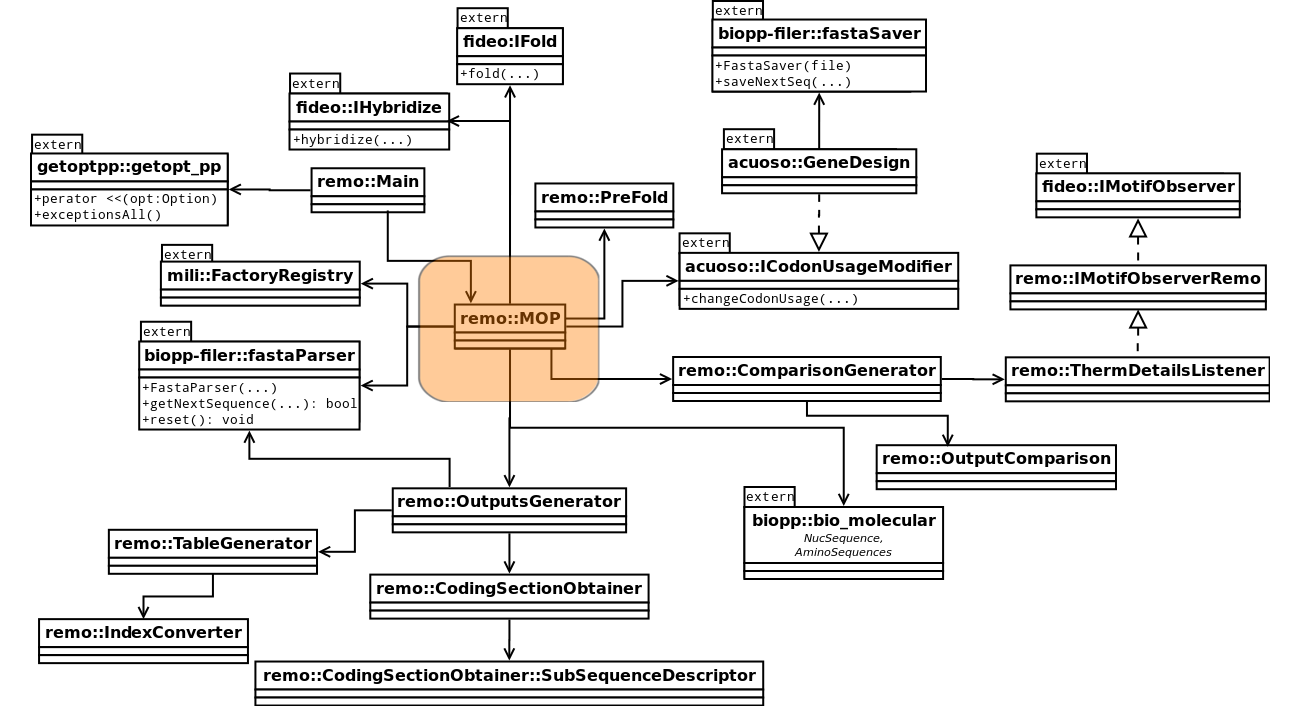
\includegraphics[scale=.25]{images/emptyClass2.png}
        \end{center}
      \end{frame}  

      \begin{frame}\frametitle{\textbf{Diagrama de Clases (Cont.)}}
        \begin{center}
          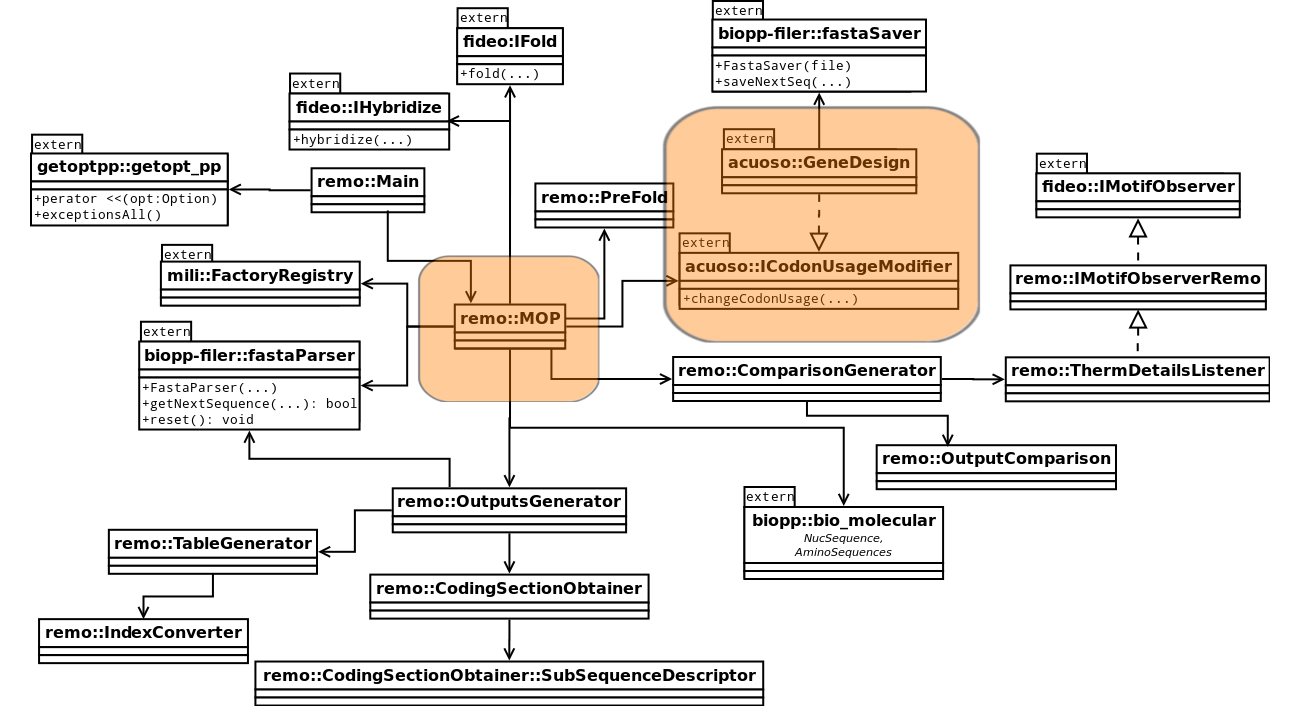
\includegraphics[scale=.25]{images/emptyClass3.png}
        \end{center}
      \end{frame}  

      \begin{frame}\frametitle{\textbf{Diagrama de Clases (Cont.)}}
        \begin{center}
          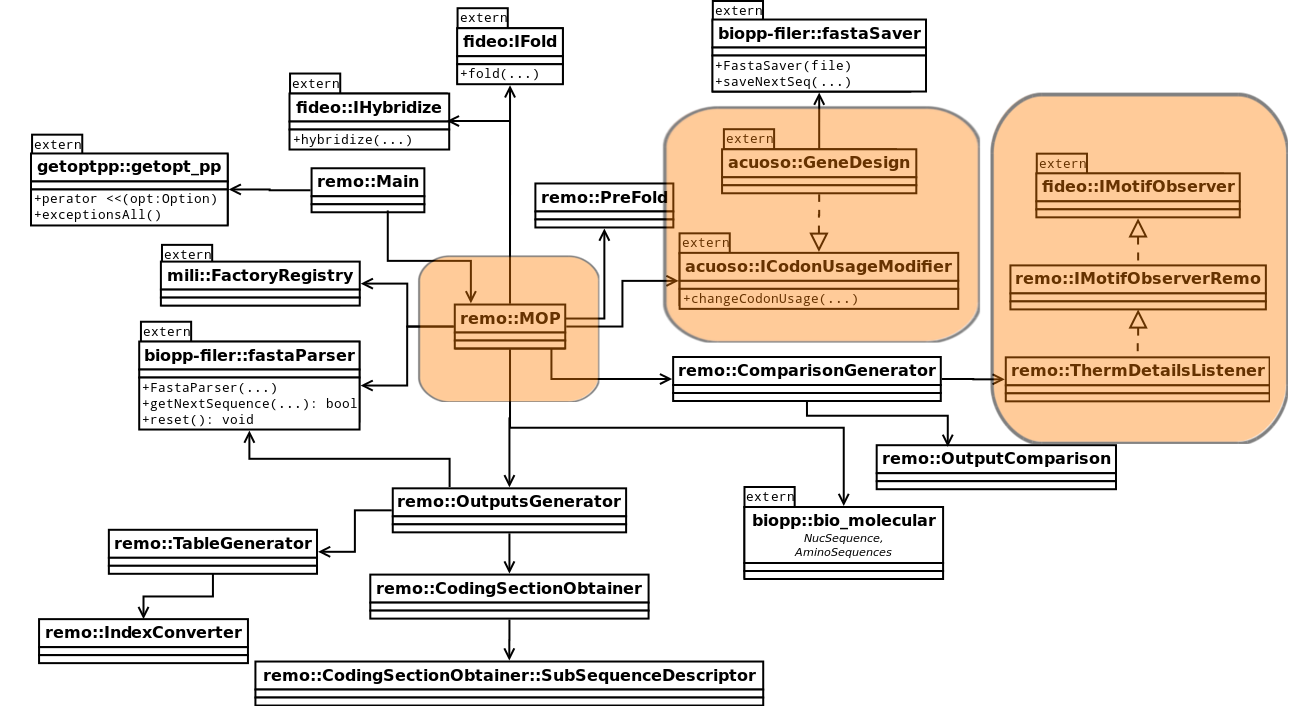
\includegraphics[scale=.25]{images/emptyClass4.png}
        \end{center}
      \end{frame}  

      \begin{frame}\frametitle{\textbf{Librerías Implementadas}}
        \begin{center}
          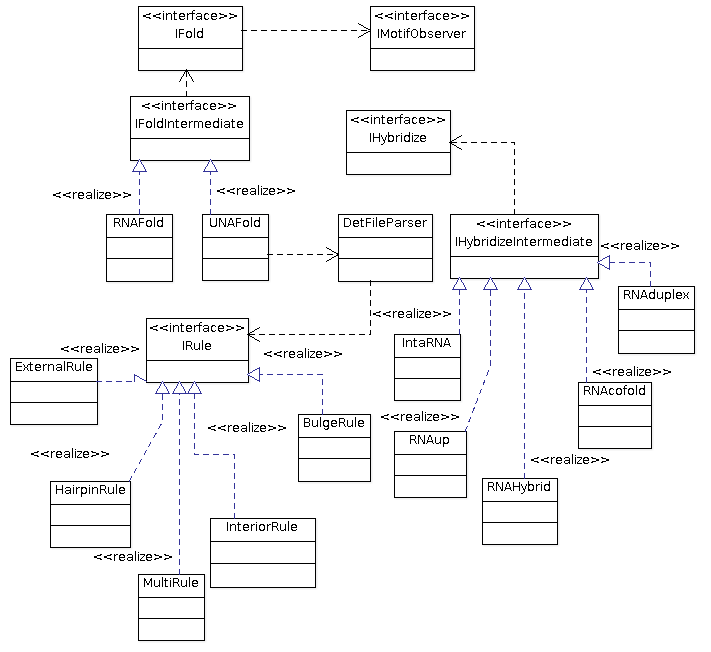
\includegraphics[scale=.3]{images/fideoInterface.png}
        \end{center}
      \end{frame}  

      \begin{frame}\frametitle{\textbf{Librerías Implementadas}}
        \begin{center}
           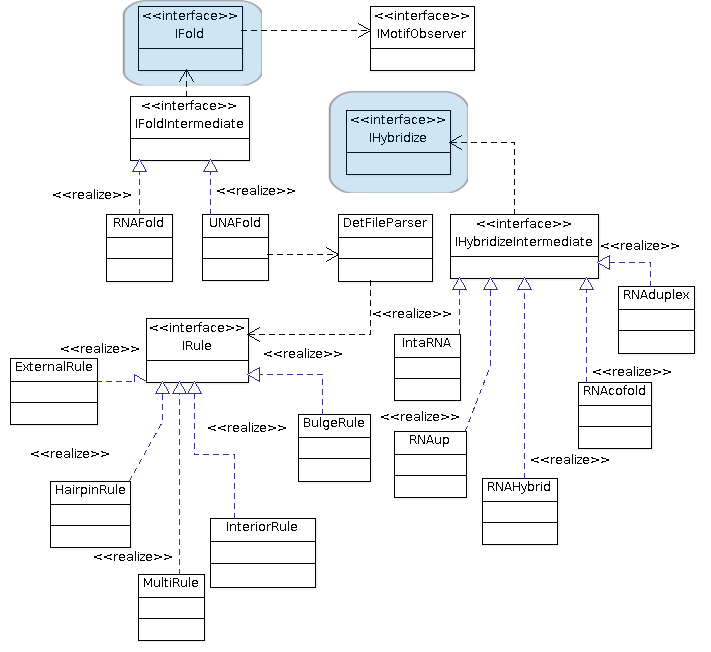
\includegraphics[scale=.3]{images/fideoInterface2.png}
        \end{center}
      \end{frame}

      \begin{frame}\frametitle{\textbf{Librerías Implementadas}}
        \begin{center}
          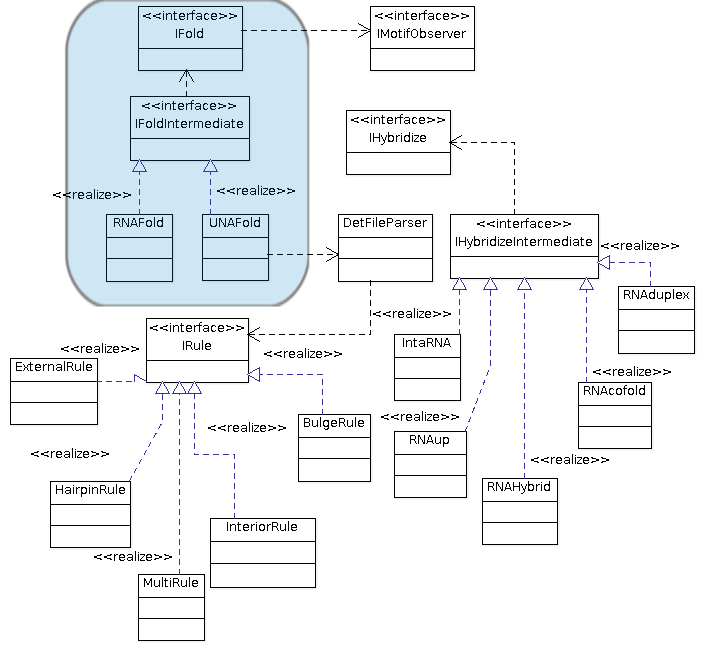
\includegraphics[scale=.3]{images/fideoInterface3.png}
        \end{center}
      \end{frame}

      \begin{frame}\frametitle{\textbf{Librerías Implementadas}}
        \begin{center}
          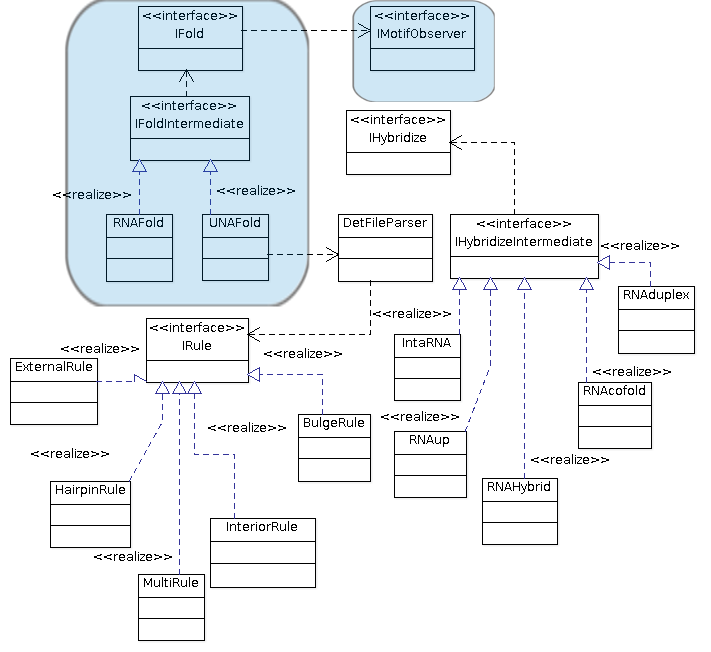
\includegraphics[scale=.3]{images/fideoInterface4.png}
        \end{center}
      \end{frame}

      \begin{frame}\frametitle{\textbf{Librerías Implementadas}}
        \begin{center}
          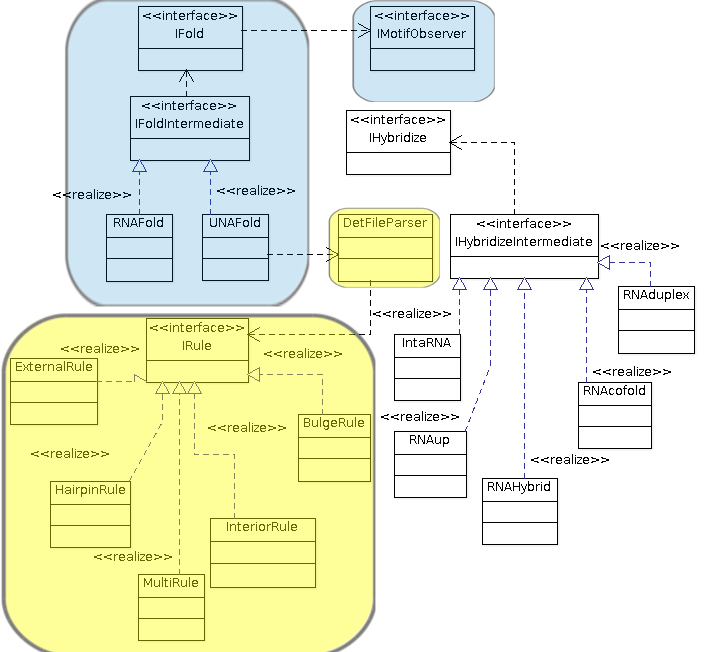
\includegraphics[scale=.3]{images/fideoInterface5.png}
        \end{center}
      \end{frame} 

  \subsection{Implementación} 
      \begin{frame}
        \frametitle{\textbf{Dependencias}}
        \begin{block}{Algunas de ellas son:}
          \begin{itemize}
            \item mili
            \item biopp 
            \item biopp-filer
            \item fud
          \end{itemize}  
        \end{block}          
        \hspace*{1.7cm}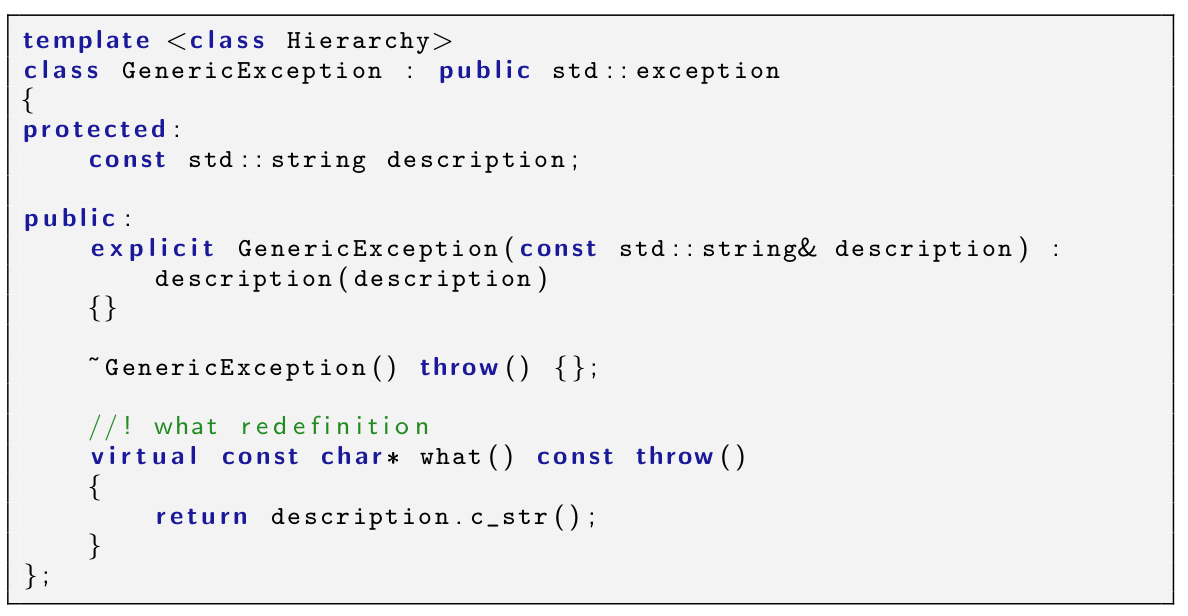
\includegraphics[scale=.18]{images/exampleMili.png}
      \end{frame}    
      
  \begin{frame}\frametitle{\textbf{Métricas de Código}}    
    \begin{table}[!htf]
    \rowcolors{2}{verde!20}{verde!5}
    \begin{tabular}{|l|r|r|r|r|c|}
    \hline
    \multicolumn{2}{|c|}{Files} & \multicolumn{3}{|c|}{Line Types} & \hspace{0.2cm}\% \\
    \hline
    \textbf{Type} & \textbf{Count} & \textbf{Blank} & \textbf{Comment} & \textbf{Source} & \small{\textbf{\#Comms./Tot.}}\\
    \hline
    \texttt{C++ source} & 10 & 161 & 553 & 1108 & 33.2 \\
    \hline
    \texttt{C++ header} & 11 & 150 & 757 & 273 & 73.4 \\
    \hline
    \textbf{Total}      & 21 & 311 & 1310 & 1381 & 48.6 \\
    \hline
    \end{tabular}    
    \end{table}
    \hspace*{3.5cm}Métricas CLOC para \textbf{Remo}.

    \begin{table}[!htf]
    % \begin{center}
    \rowcolors{2}{verde!20}{verde!5}
    \begin{tabular}{|l|r|r|r|r|c|}
    \hline
    \multicolumn{2}{|c|}{Files} & \multicolumn{3}{|c|}{Line Types} & \hspace{0.2cm}\% \\
    \hline
    \textbf{Type} & \textbf{Count} & \textbf{Blank} & \textbf{Comment} & \textbf{Source} & \small{\textbf{\#Comms./Tot.}}\\
    \hline
    \texttt{C++ source} & 10   &    161  &     344   &    967 & 26.2 \\
    \hline
    \texttt{C++ header} & 20   &    243  &    1222   &    603 & 66.9 \\
    \hline
    \textbf{Total}      &  30  &     404 &     1566  &    1570 & 49.9 \\
    \hline
    \end{tabular}
    \end{table}
    \hspace*{3.5cm} Métricas CLOC para \textbf{fideo}.
  \end{frame}

  \begin{frame}\frametitle{\textbf{Métricas de Código (cont)}}    
    \begin{table}[!htf]
      \begin{tabular}{|l|l|l|l|l|l|}
      \hline
      \textbf{Component} & \textbf{Count} & \textbf{Blank} & \textbf{Comment} & \textbf{Source} & \small{\textbf{\#Comms./Tot.}}\\
      \hline
      r-emo           & 21 & 311  & 1310  & 1381 & 48.6 \\ \hline
      fideo           & 30 & 404  & 1566  & 1570 & 49.9 \\ \hline
      acuoso          & 7  & 72   & 319   & 272  & 53   \\ \hline
      etilico         & 8  & 82   & 327   & 297  & 52.4 \\ \hline
      r-emo client    & 4  & 45   & 152   & 133  & 0.46 \\ \hline
      r-emo server    & 8  & 104  & 272   & 531  & 0.33 \\ \hline
      \textbf{Total}  & \textbf{78} & \textbf{1018} & \textbf{3946}  & \textbf{4184} & \textbf{0.48} \\ \hline
      \end{tabular}
      \end{table}
      \hspace*{3.5cm}\textbf{Resúmen Código producido}.
  \end{frame} 

  \begin{frame}
    \frametitle{\textbf{Comentarios Doxygen}}    
    \hspace*{.6cm}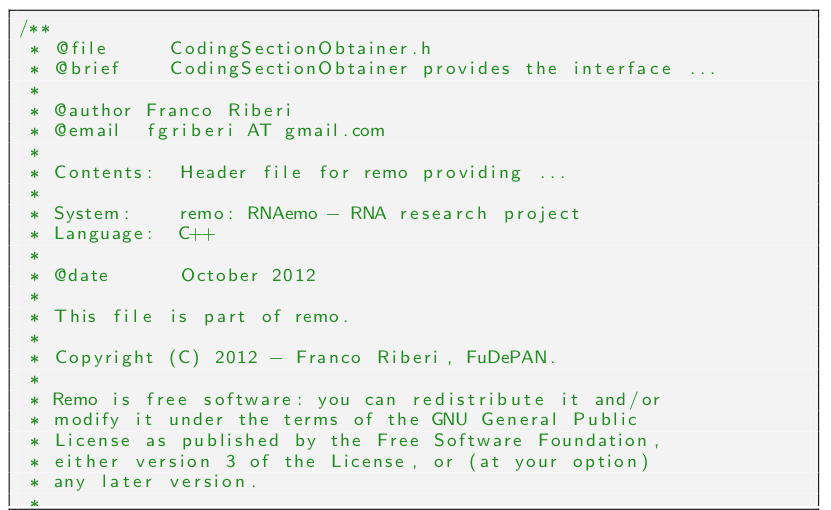
\includegraphics[scale=.35]{images/doxygen.png}
  \end{frame}   